
\documentclass[12pt]{article}

% margin left and right with \setlength{\itemindent}{-.5in} %
\usepackage{enumitem}

% leave out section numbers in subsection numbering %
\usepackage[T1]{fontenc}
\renewcommand*\thesubsection{\arabic{subsection}}


% include Roman numerals for sections %
\renewcommand{\thesection}{\Roman{section}}
%Roman numerals for subsections like this \renewcommand{\thesubsection}{\Roman{subsection}}%
% include the package of the color%
\usepackage[usenames, dvipsnames]{color}
\usepackage[english]{babel}
\usepackage[utf8x]{inputenc}
\usepackage{amsmath}
\usepackage{graphicx}
\usepackage{subfiles}

%define your own color %
\definecolor{mygray}{gray}{0.9}
\begin{document}
	\listoffigures
	\title{Chapter 2 : Analysis and specification of requirements}
	\maketitle
	
	\section{Introduction}
	Being the first in the development cycle of the project, this phase is the most
	important. Indeed, it is during this period that the needs of the user are identified and specified. These requirements also represent the functionalities that should be present in the application, which also makes it possible to validate the application as the development progresses.
	\section{Actors Identification}
	\textbf{MassTer Insight web Application }was mainly designed to be used by \textbf{Data Analysts }in MMM agencies, which is the case of \textbf{MASS Analytics}, \textbf{Media Agencies }that have a MMM division, and \textbf{Advertisers }who have an in-house MMM team.
	
	\clearpage
	\newpage
	
	
	\section{Requirement Analysis}

	\subsection{Functional Requirements}
     
	These functional requirements express the expectations of different users for the product to be produced.
	\\
	\\
	In this part, we present the different functionalities and services that the application must ensure.
	
	CONNECT TO SERVER
	\begin{itemize}
		\setlength{\itemindent}{+.5in}
		\item \textbf{Connect To MassTer Server : } 
	\end{itemize}
	
	LOAD PROJECT
	\begin{itemize}
		\setlength{\itemindent}{+.5in}
     	\item \textbf{Load MassTer Insight Project : } 
    \end{itemize}	
 
 	MANAGE REPORT
 		\begin{itemize}
 			\setlength{\itemindent}{+.5in}
 			\item \textbf{Available Reports : } 
 			\item \textbf{Save a Report : }
 			\item \textbf{Remove a Report : }
 			\item \textbf{Load a Report : } 
 			\item \textbf{Available Channel : } 
 			\item \textbf{Seasonality Index Per Month : }
 			\item \textbf{Ignore Preset Laydown : }
 			\item \textbf{Budget Tolerance : }
 			\item \textbf{Revenue Tolerance : }
 			\item \textbf{Max Iteration  : }
 			\item \textbf{Max Iteration  : }
 			\item \textbf{Budget Range : }
 			\item \textbf{Total Budget : }
 			\item \textbf{Min Target : }
 			\item \textbf{Select Channel : }
 			\item \textbf{Max budget/Min Target/Set Budget per Channel : }
 	\end{itemize}
 
  	UPDATE
    \begin{itemize}
    	\setlength{\itemindent}{+.5in}
    	\item \textbf{Update a Report : }
   \end{itemize}

  	RUN
   \begin{itemize}
   	   \setlength{\itemindent}{+.5in}
 	   \item \textbf{Run new scenario : }
   \end{itemize}

    \clearpage
    \newpage

	\subsection{Non-Functional Requirements}
	
	\clearpage
	\newpage
	
	\section{Use Case Diagrams}
	\subsection{Global Use Case Diagram}
	\clearpage
	\newpage
	\begin{figure}[h]
		\centering
		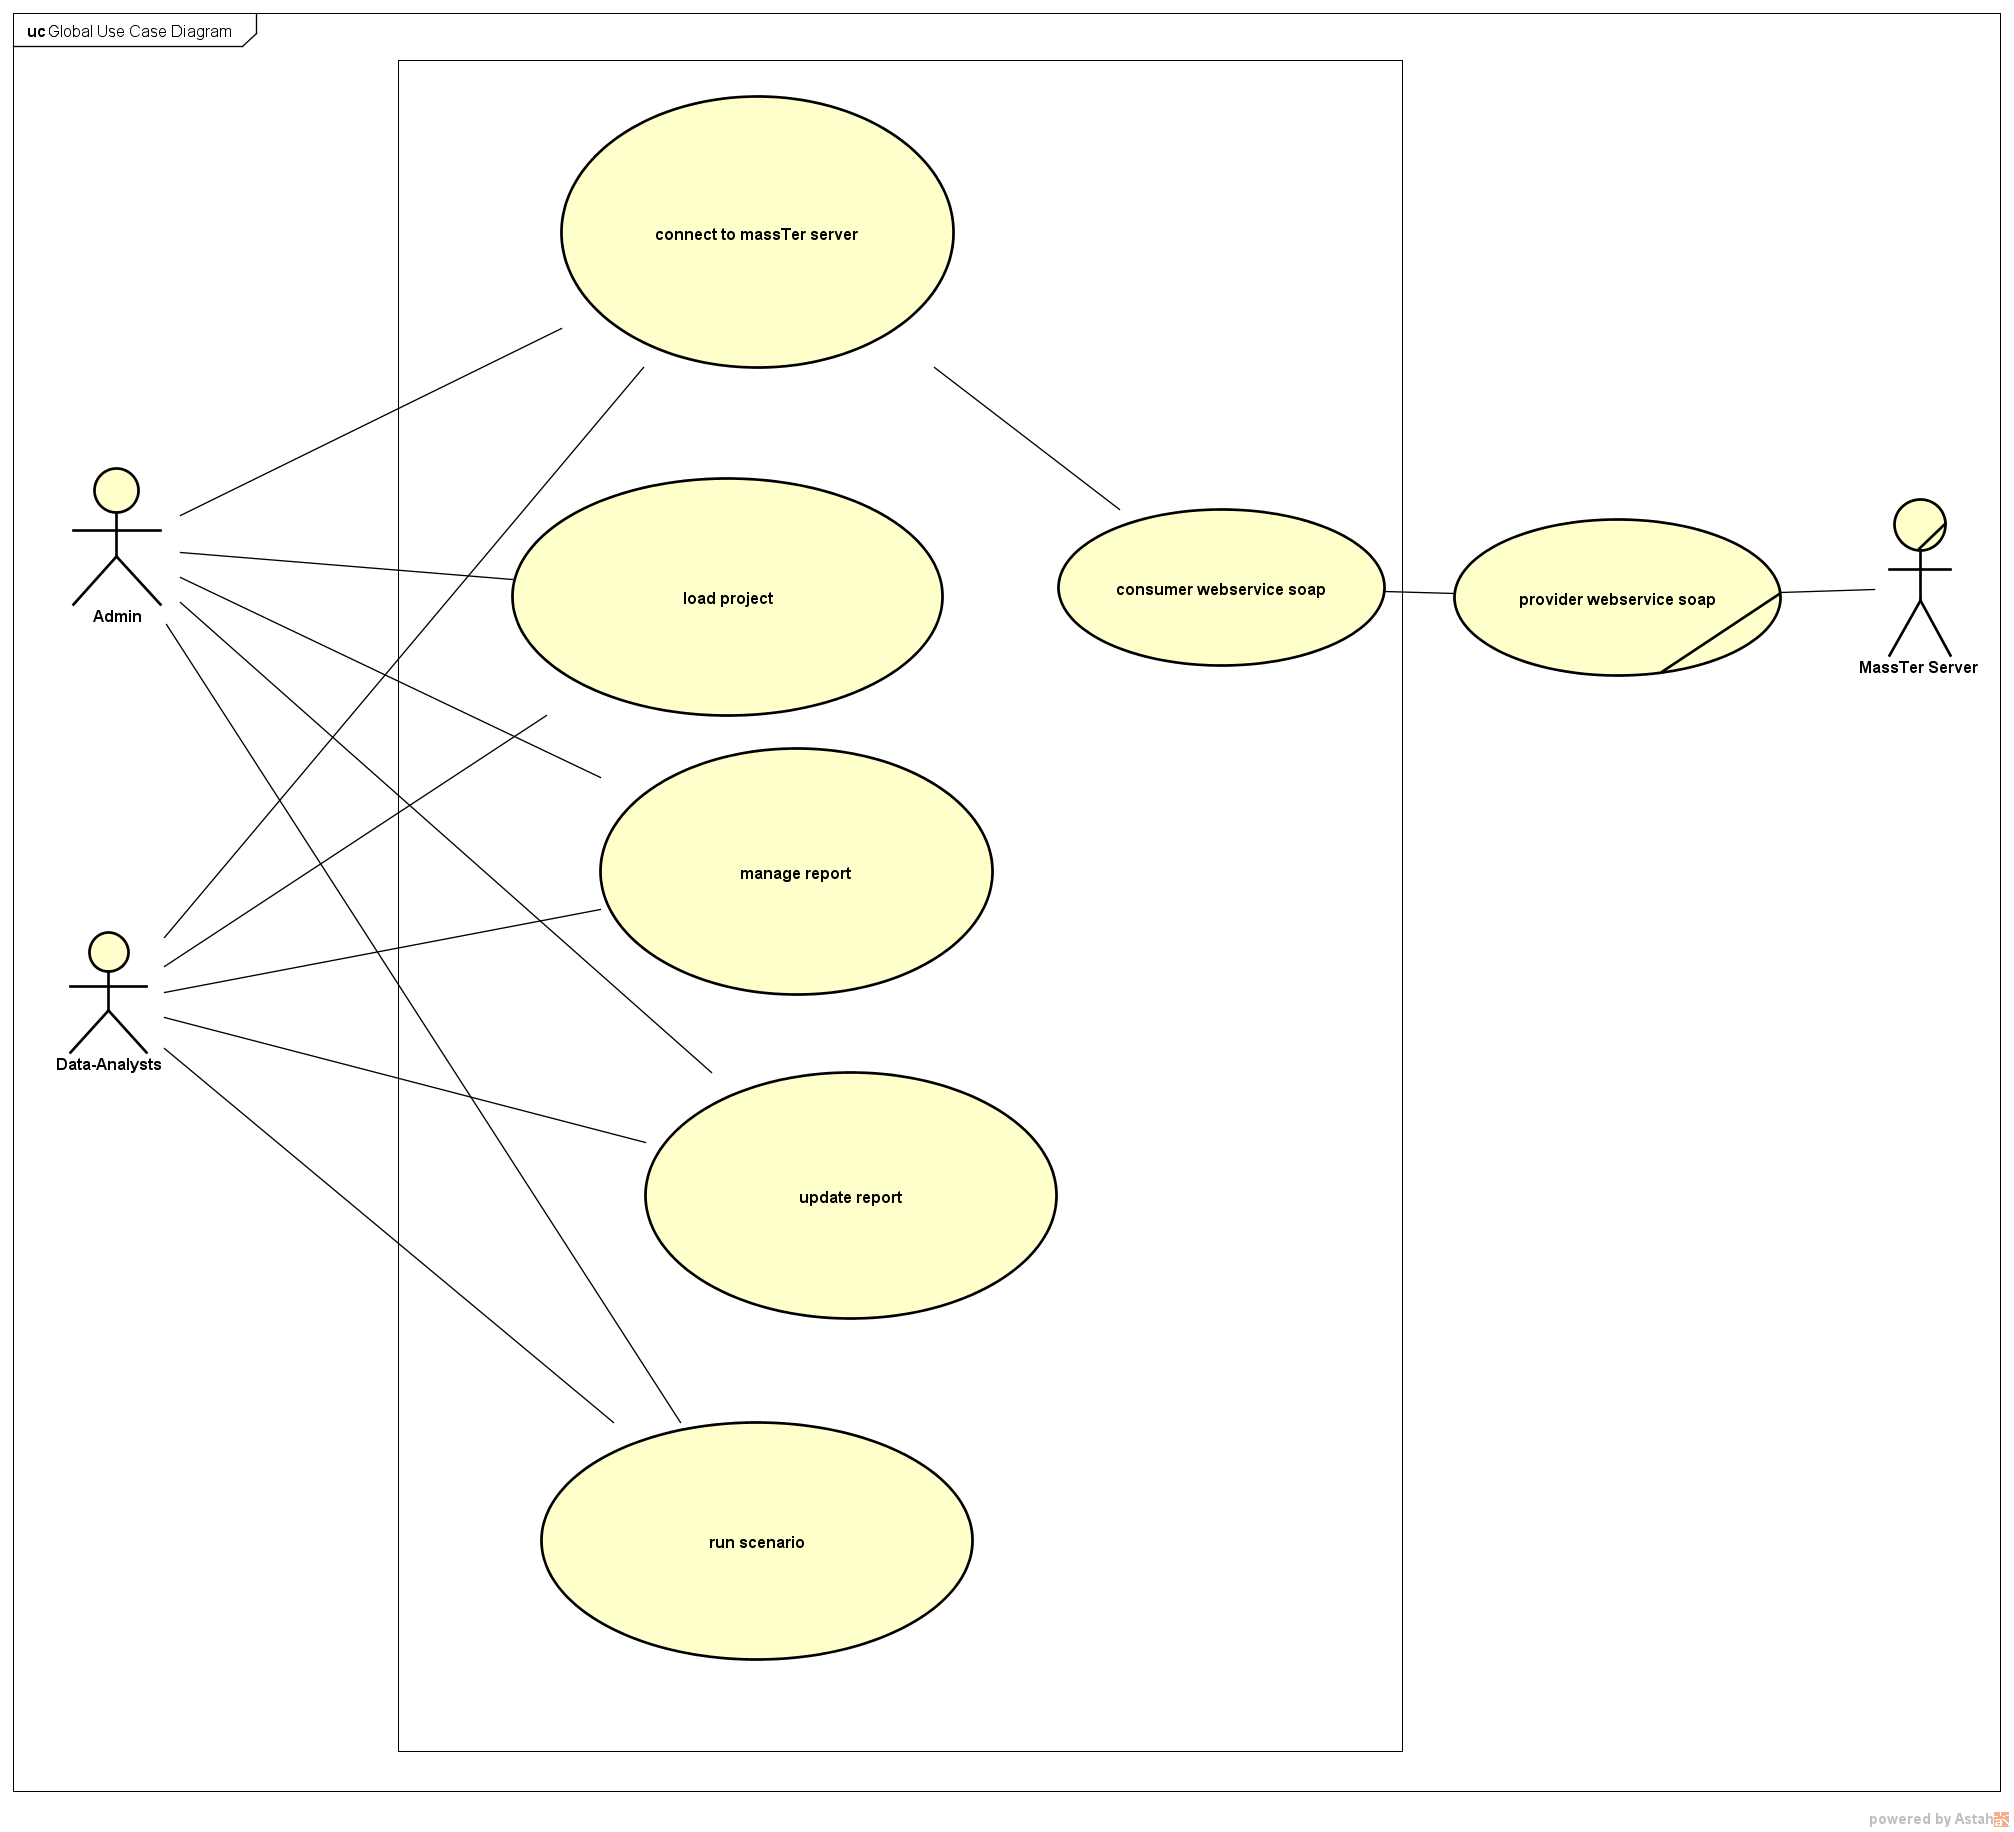
\includegraphics[width=1.0\textwidth]{GlobalUseCaseDiagram.png}
		\caption{Global Use Case Diagram}
		
	\end{figure}

\clearpage
\newpage


	\subsection{Detailed Use Case Diagrams}
	\clearpage
	\newpage
	 \subsubsection{connect to MassTer Server}
	 	\begin{figure}[h]
	 	\centering
	 	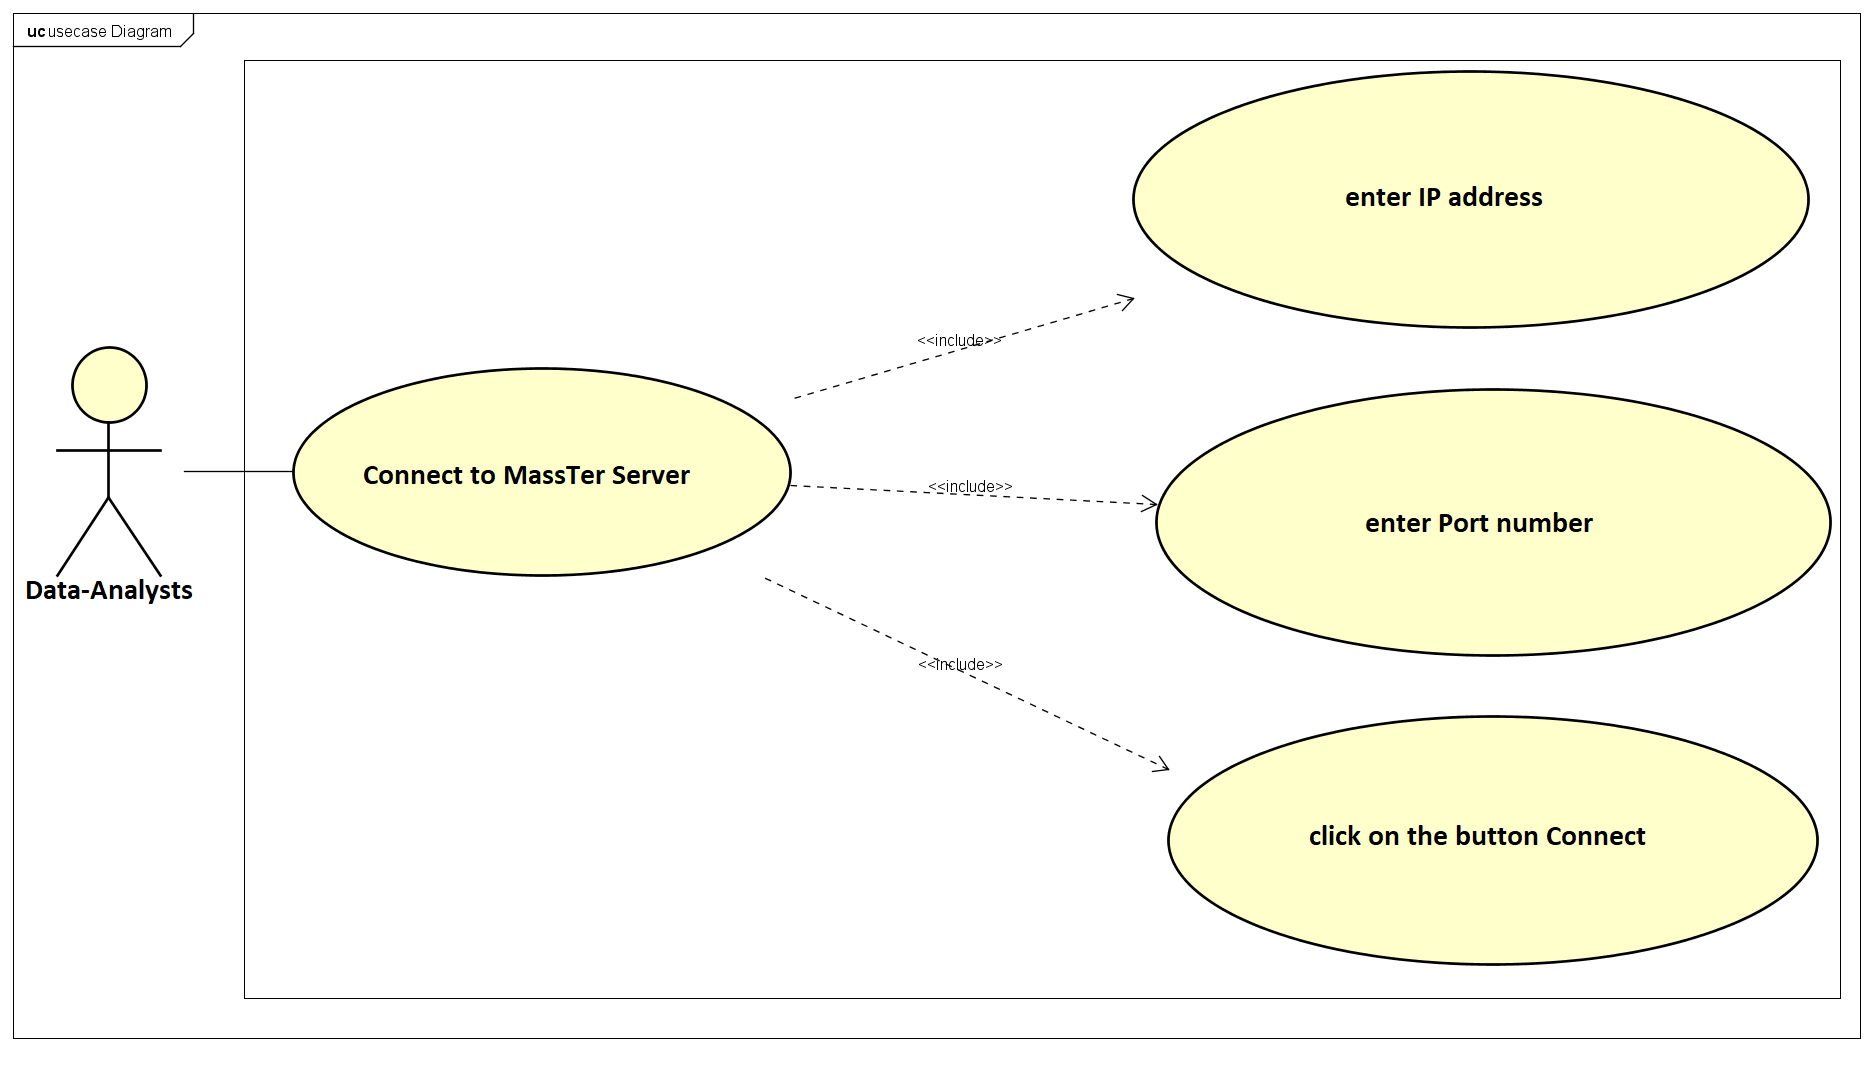
\includegraphics[width=1.0\textwidth]{connectToMassTerServer.png}
	 	\caption{connect to MassTer Server Use Case Diagram}
	 	
	 \end{figure}
 \clearpage
 \newpage
	 \subsubsection{consume webService soap}
	 	 	\begin{figure}[h]
	 	\centering
	 	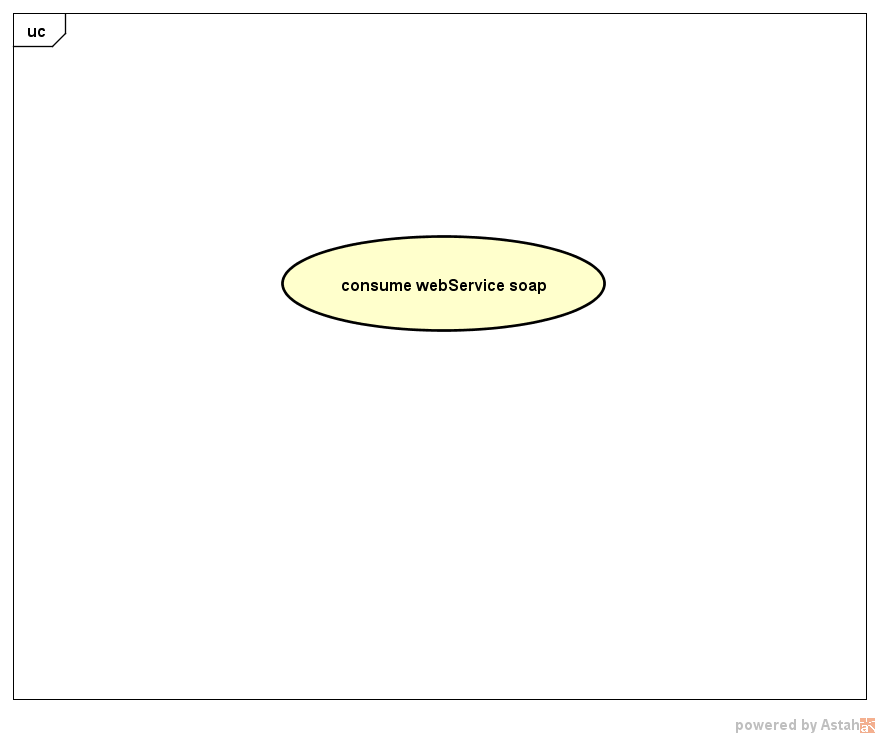
\includegraphics[width=1.0\textwidth]{consumewebServicesoap.png}
	 	\caption{consume webService soap Use Case Diagram}
	 	
	 \end{figure}
 \clearpage
 \newpage

	 \subsubsection{provide webService soap} 
	 	\begin{figure}[h]
	 	\centering
	 	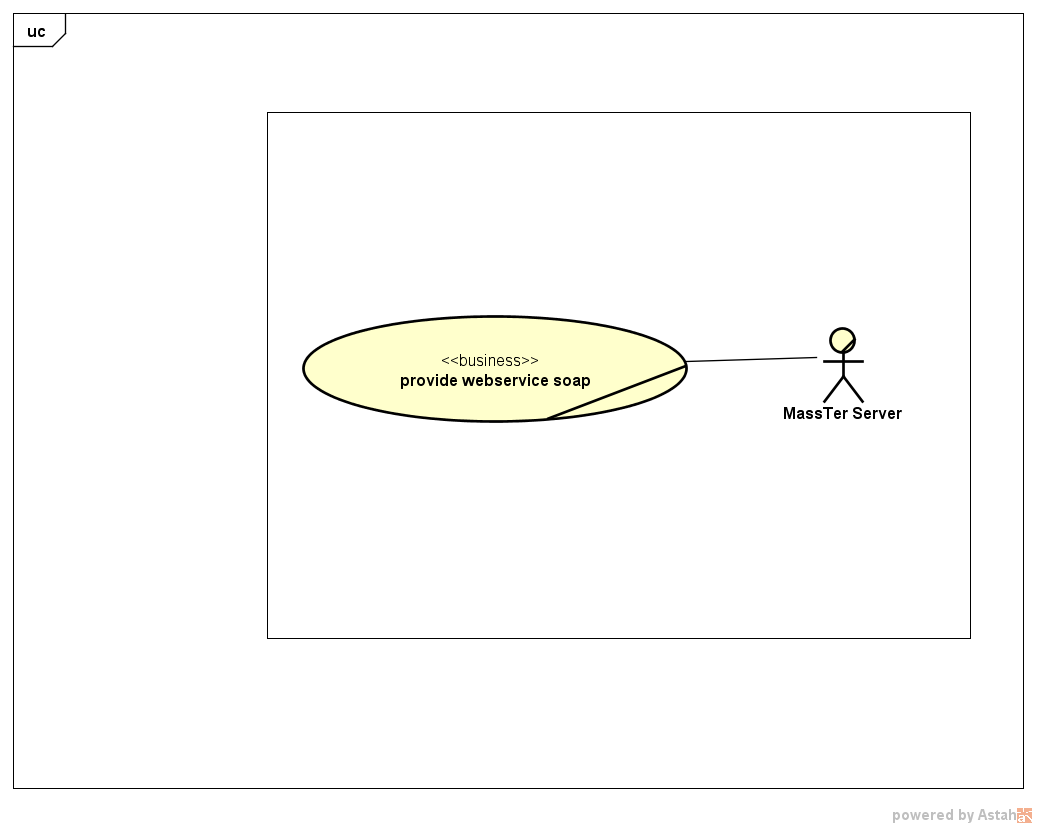
\includegraphics[width=1.0\textwidth]{provideWebServiceSoap.png}
	 	\caption{provide webService soap Use Case Diagram}
	 	
	 \end{figure}
 \clearpage
 \newpage
	 \subsubsection{load project}
	 	\begin{figure}[h]
	\centering
	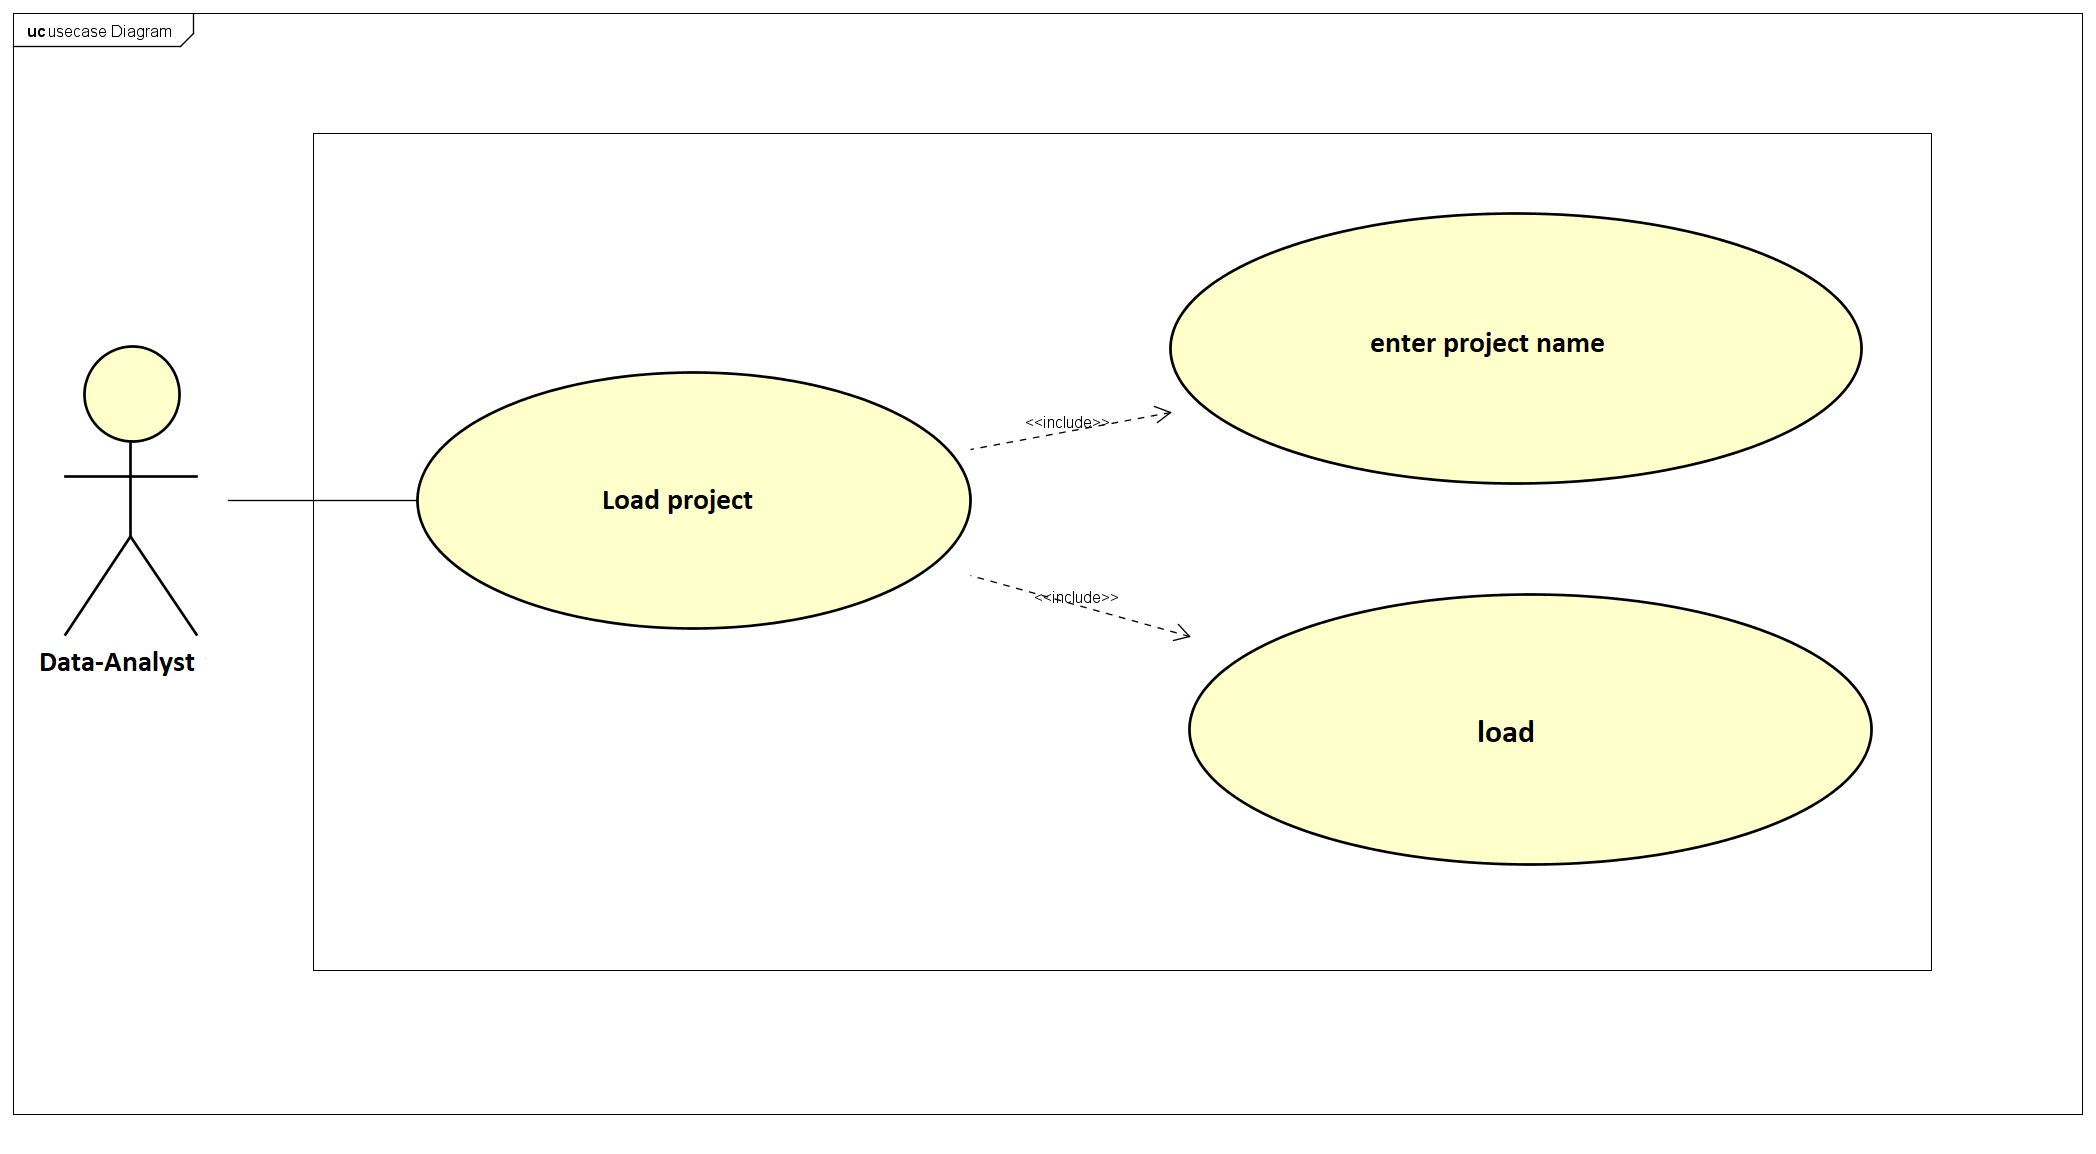
\includegraphics[width=1.0\textwidth]{loadProject.png}
	\caption{load project Use Case Diagram}
	
	\end{figure}
\clearpage
\newpage
	 \subsubsection{manage report}
	 	\begin{figure}[h]
	 	\centering
	 	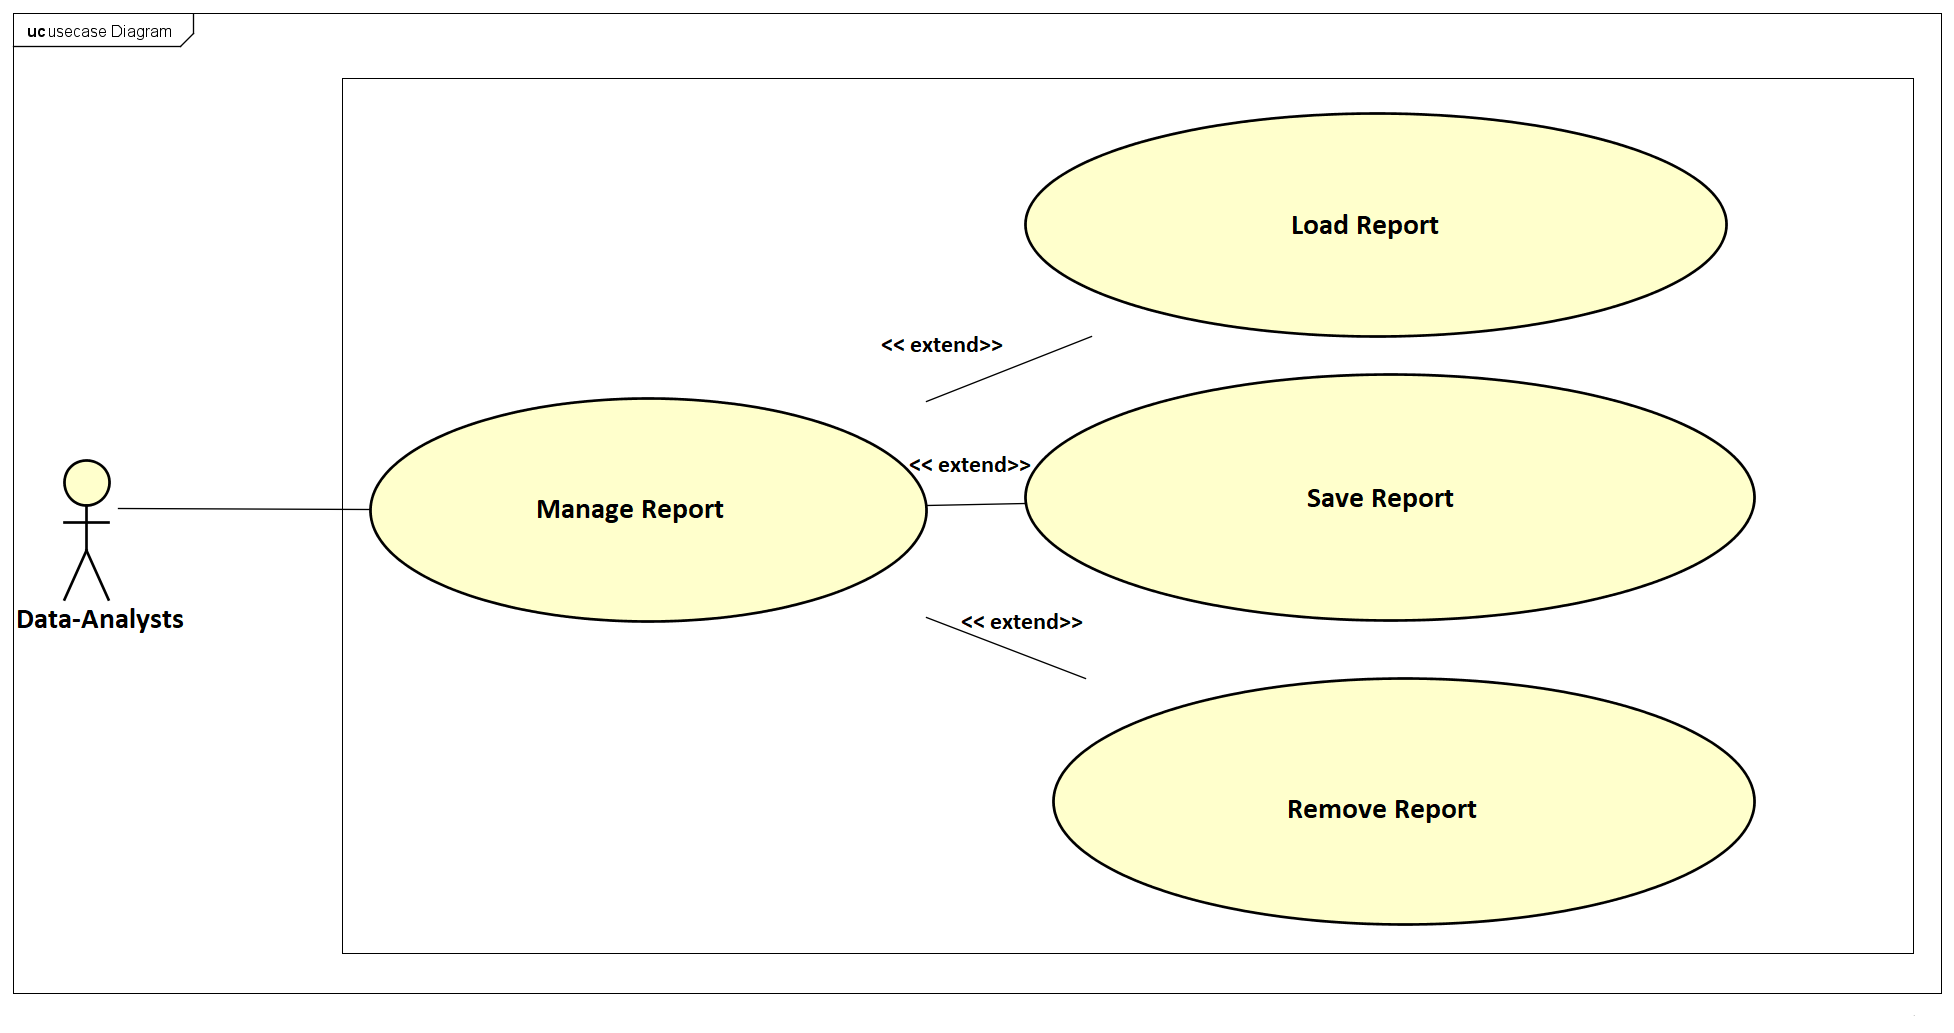
\includegraphics[width=1.0\textwidth]{manageReport.png}
	 	\caption{manage report Use Case Diagram}
	 	
	 \end{figure}
 \clearpage
 \newpage
	 \subsubsection{update settings}
	 	\begin{figure}[h]
	 	\centering
	 	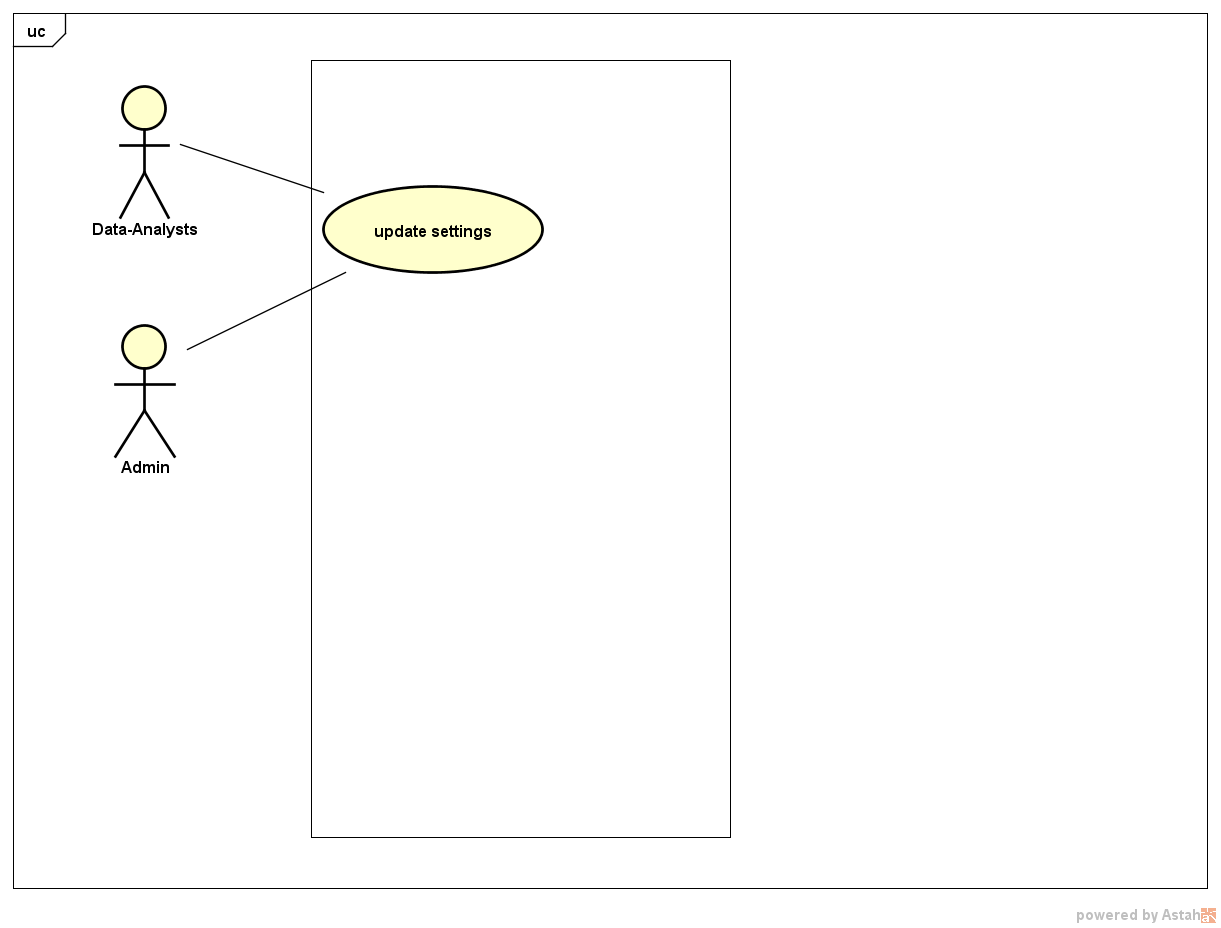
\includegraphics[width=1.0\textwidth]{updateSettings.png}
	 	\caption{update settings Use Case Diagram}
	 	
	 \end{figure}
 \clearpage
 \newpage
	 \subsubsection{run scenario}
	 	\begin{figure}[h]
	 	\centering
	 	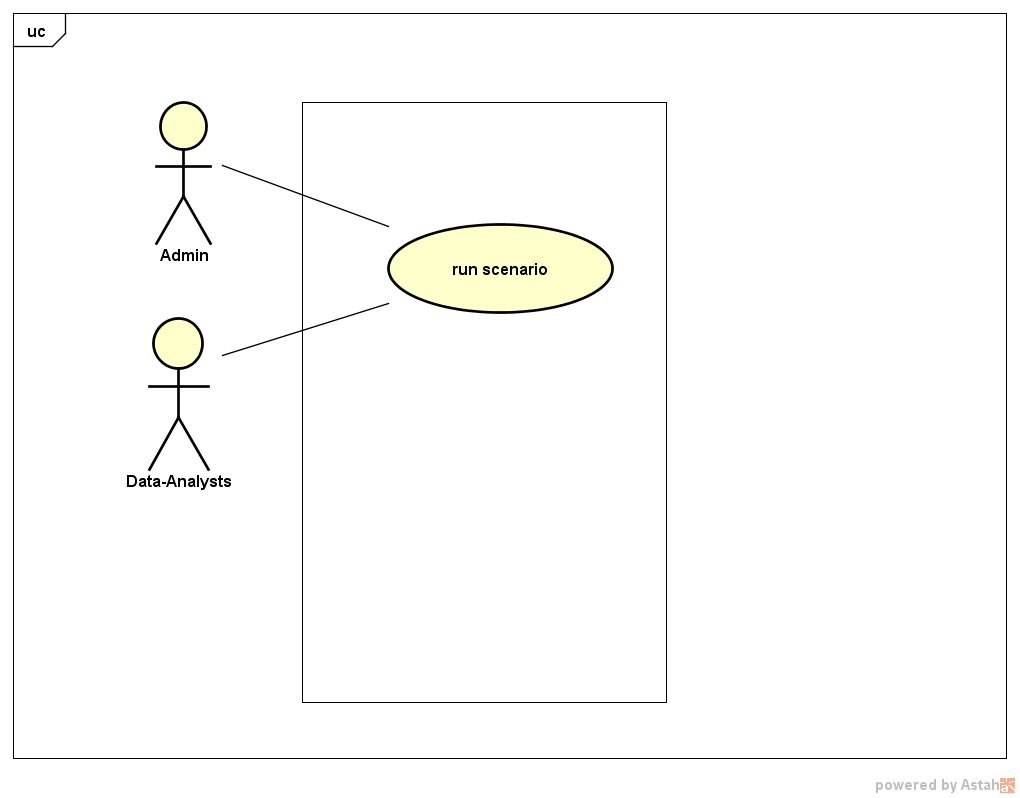
\includegraphics[width=1.0\textwidth]{runScenario.png}
	 	\caption{run scenario Use Case Diagram}
	 	
	 \end{figure}
	
	
	\clearpage
	\newpage
	
	\section{Conclusion}
	
\end{document}